%!TEX root = lec07_documents.tex

\begin{frame}{Approaches for storing XML}

\begin{itemize}[-]
\item File System: keep documents as text files.
\item Native XML Store.
\begin{itemize}[-]
\item Implement persistent data structures to represent the XML (DOM) tree.
\end{itemize}
\item Inside a Relational DBMS: re-use existing storage, indexing, (and querying) systems.
\begin{itemize}[-]
\item String or BLOB attribute.
\item \emph{XML Mappings}.
\begin{itemize}[$\star$]
\item Schema-based.
\item Structure-based.
\end{itemize}
\end{itemize}
\end{itemize}
\end{frame}


\begin{frame}{XML documents in the File System}

\begin{itemize}[-]
\item Advantages:
\begin{itemize}[-]
\item Simplicity. 
\item Re-using existing I/O layer (and file-level locking) provided by the Operating System.
\end{itemize}

\item Disadvantages:
\begin{itemize}[-]
\item Document (and data therein) is exposed to \alert{any user} and/or \alert{any tool} (e.g., a text editor) that has access to the directory where the documents are stored.
\item Duplicated efforts: logging, concurrency control, back-ups, security, etc. are done outside the DBMSs.
\item Hard to coordinate queries that involve relational (in-DBMS) and XML (out-of-DBMS) data.
\end{itemize}
\end{itemize}
\end{frame}

\begin{frame}{Native XML Stores}

These systems are tailored for working with XML documents of any size (typically, they support up to a few GB per document), supporting queries and update natively.

In a sense, these are highly I/O optimized implementations of tree data-structures.

Some systems listed on Wikipedia (circa 2019):

\hspace*{-20pt}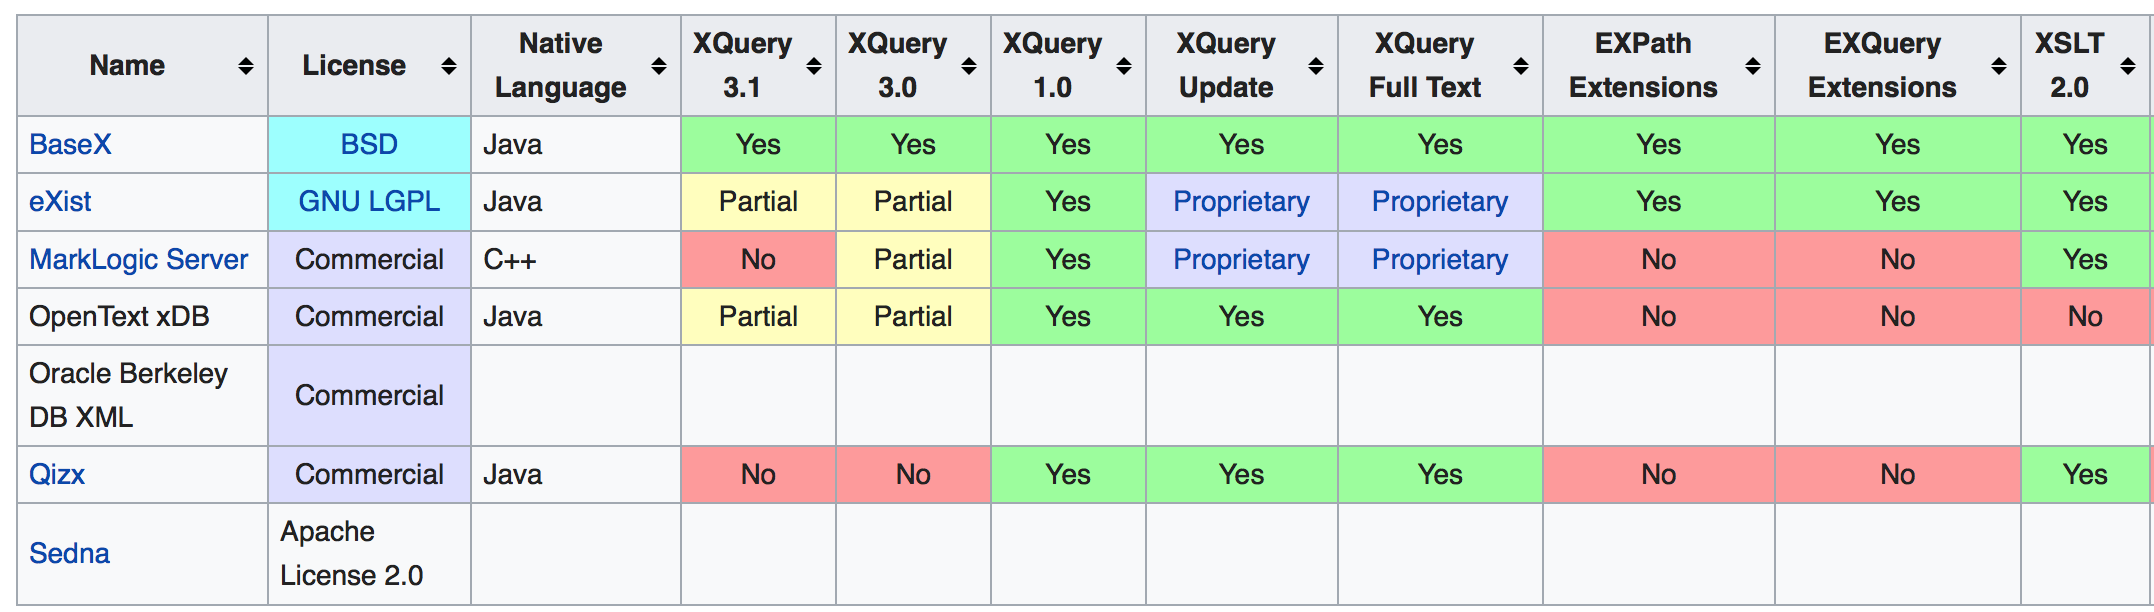
\includegraphics[width=1.15\textwidth]{figures/native_XML_stores.png}
\end{frame}


\begin{frame}{Native XML Stores}

Full fledged native stores combine the functionality of a file server (e.g., WebDAV support) and a Web server (HTTP support) with that of a database management system (e.g., command-line SQL and API support for queries and updates, indexing, transaction management, etc.).

For commercial reasons, XML Stores must also support SQL systems to be successful. 

Some strategies:
\begin{itemize}[-]
\item Exporting XML data as relational views that can be read and modified by an external application.
\item Offering native SQL support.
\end{itemize}
\end{frame}

\begin{frame}{Oracle XML DB}
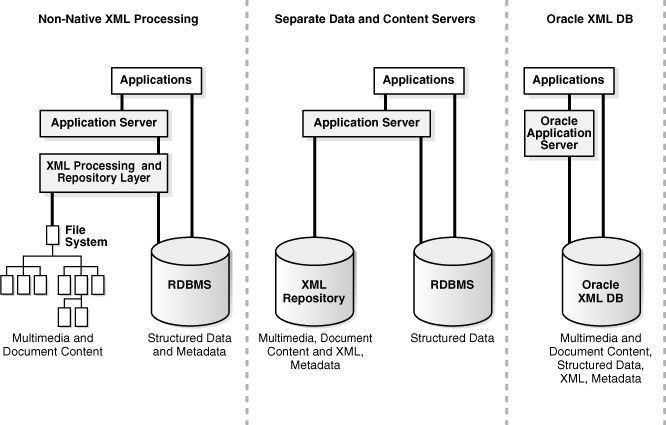
\includegraphics[width=\textwidth]{figures/Oracle_XMLDB.png}

\footnotesize Source \url{https://docs.oracle.com/cd/B19306_01/appdev.102/b14259/xdb01int.htm}
\end{frame}


\begin{frame}
\begin{center}
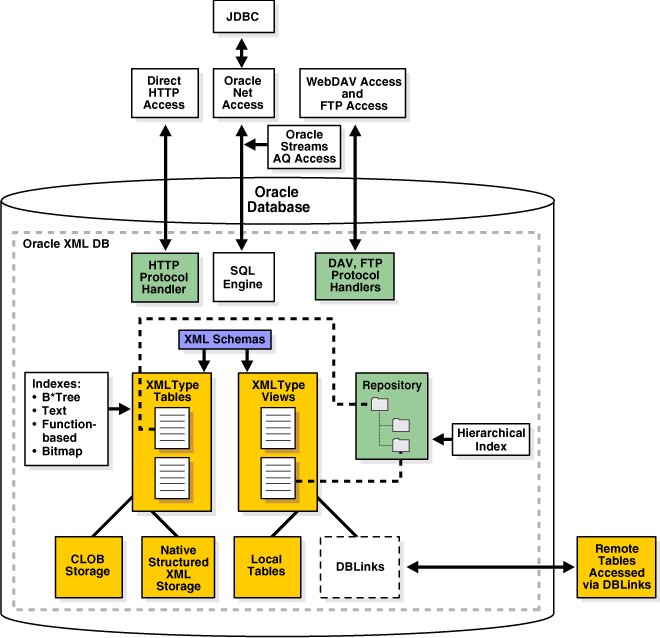
\includegraphics[width=0.75\textwidth]{figures/Oracle_XMLDB2.png}
\end{center}
\footnotesize Source \url{https://docs.oracle.com/cd/B19306_01/appdev.102/b14259/xdb01int.htm}
\end{frame}

\begin{frame}{BaseX}

BaseX was started by Christian Grün at the University of Konstanz in 2005. In 2007, BaseX went open source and has been BSD-licensed since then.

Fully developed in Java.

Supports XPath, XQuery 3.1, WebDAV, and various API/connector protocols.

Concurrency control:
\begin{itemize}[-]
\item Queries run in parallel.
\item Updates run with locking.
\end{itemize}

\footnotesize Sources \url{http://basex.org} and \url{https://en.wikipedia.org/wiki/BaseX}
\end{frame}

\begin{frame}{eXist}

eXist is an open-source \alert{client/server} native XML database manager supporting all popular XML protocols, XQuery, indexing, updates, proper concurrency control, \textbf{triggers}, and more!

\vskip2em

\begin{center}
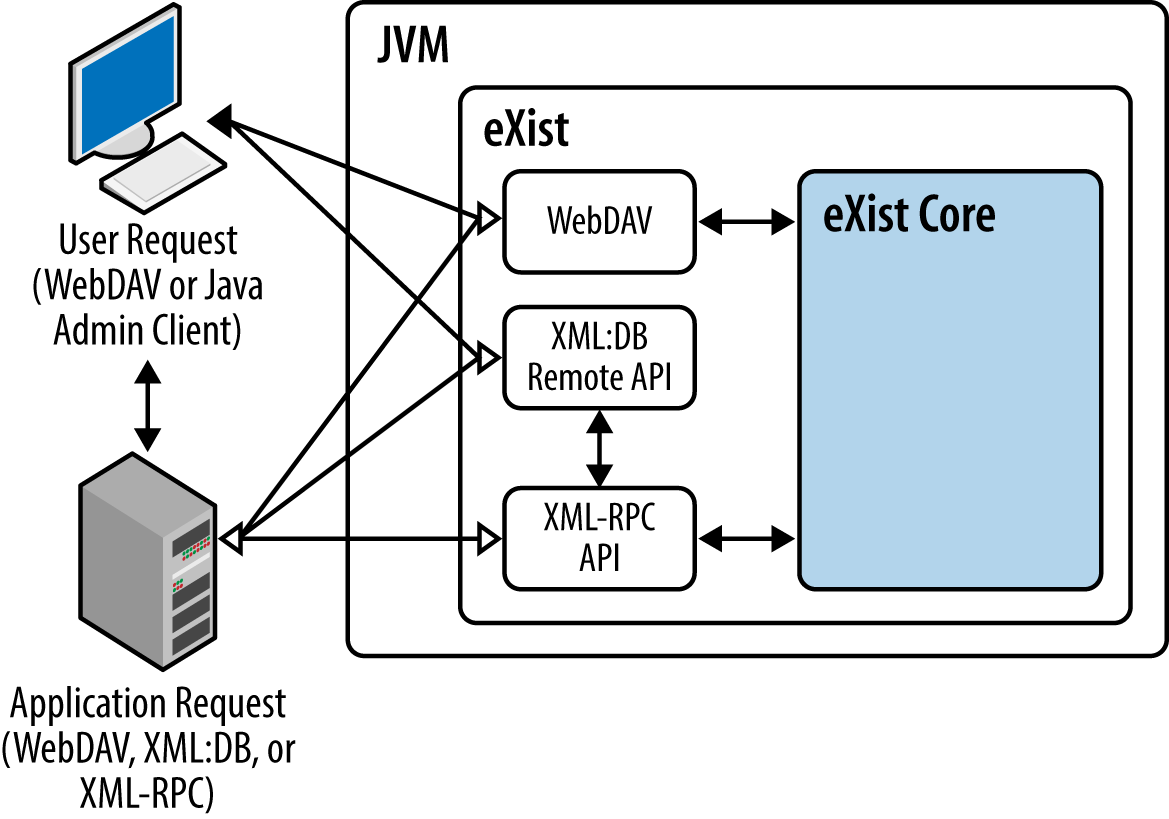
\includegraphics[width=0.6\textwidth]{figures/eXist_clientServer.png}
\end{center}

\footnotesize Source: eXist, by Retter and Siegel, O'Reilly 2014\\\url{https://learning.oreilly.com/library/view/exist/9781449337094/}
\end{frame}

\begin{frame}
\vskip1em
\begin{columns}[onlytextwidth]
\begin{column}{0.25\textwidth}

\footnotesize Source: eXist, by Retter and Siegel, O'Reilly 2014

\end{column}
\begin{column}{0.6\textwidth}
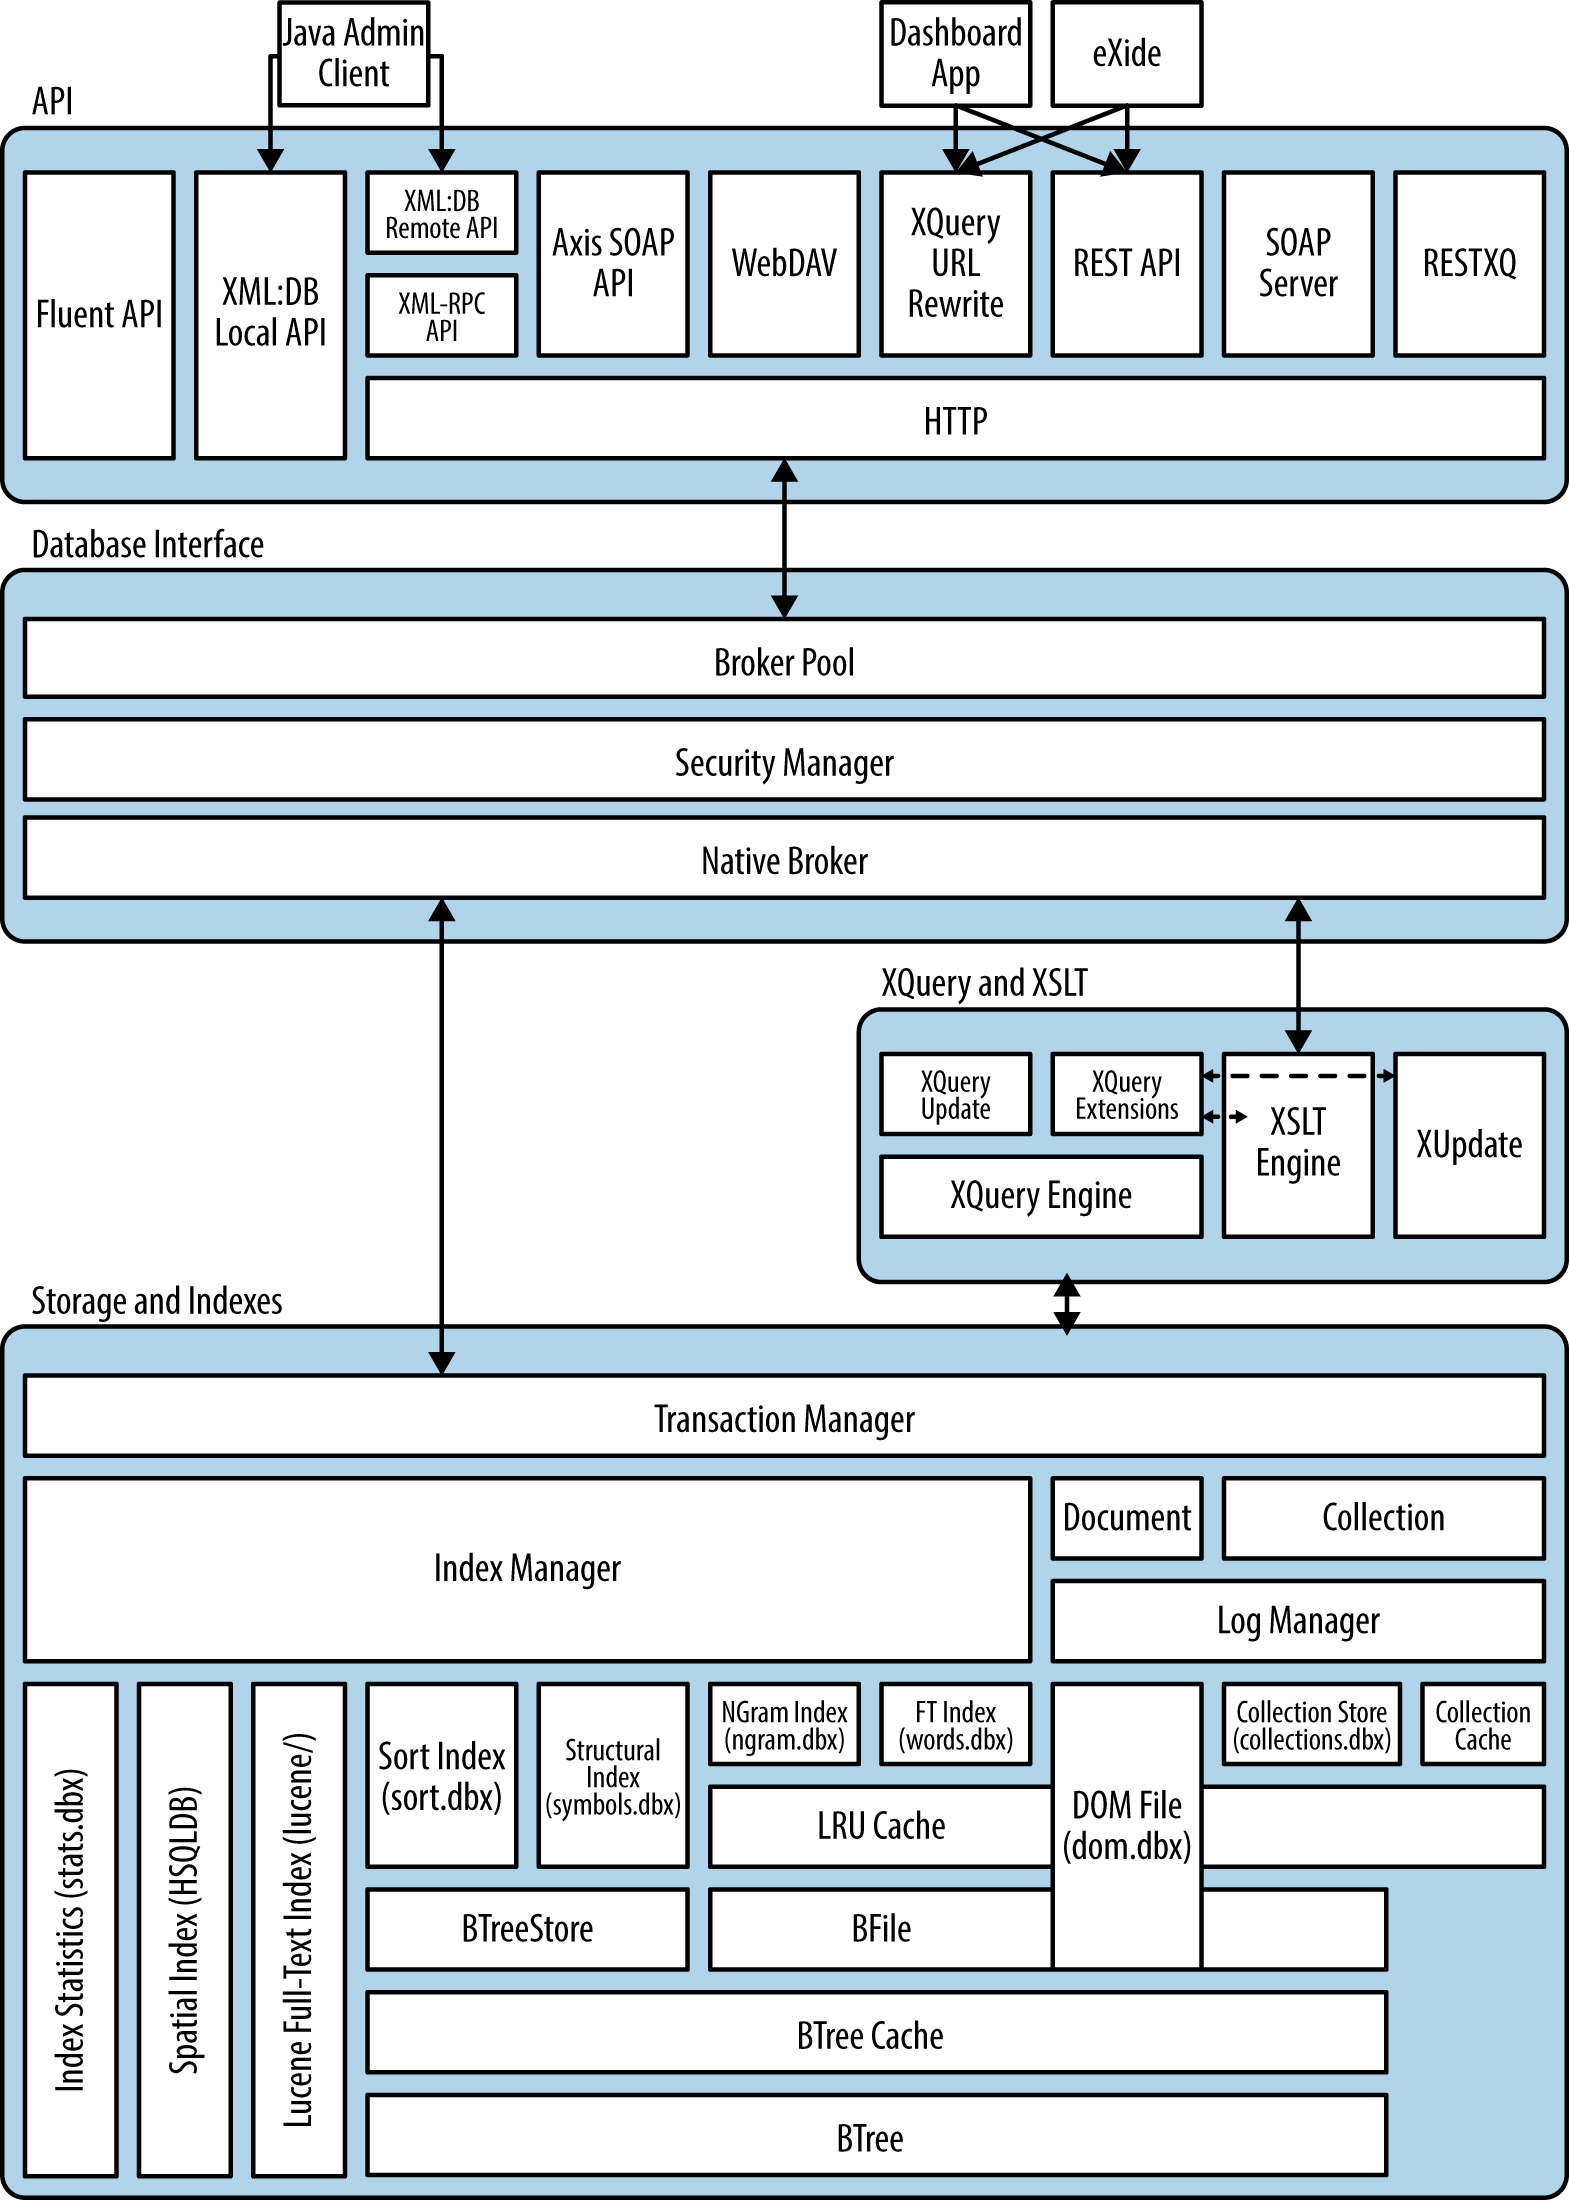
\includegraphics[width=1\textwidth]{figures/eXist_architecture.png}
\end{column}
\end{columns}
\end{frame}


\begin{frame}{Native XML Stores}

Native XML stores are a form of NoSQL that has gained much popularity since the mid-2000s, and can be used in support of document stores and Web Services.

\begin{itemize}[-]
\item Advantages:
\begin{itemize}[-]
\item Can implement optimizations specific for XML and XQuery.
\item Single application development platform.
\item ``Single Source of Truth'' for XML data: avoid fragmenting or mapping data into possibly inconsistent pieces.
\end{itemize}
\item Disadvantages:
\begin{itemize}[-]
\item Might not integrate well with existing legacy applications.
\end{itemize}
\end{itemize}
\end{frame}


\begin{frame}{RDBMS support for XML}

With the rise of native XML database management systems, many applications were ported away from RDBMSs. 

Relational vendors responded by offering support for XML within their relational products, which came in two forms: 

\begin{itemize}[-]
\item An \alert{XML data type} which can be used to store (\alert{native}ly) XML documents as attributes of a regular tuple.
\item \alert{XML Mappings}, in which XML data and queries are \alert{translated} into relational data and queries.
\end{itemize}

An industry standard, SQL/XML\footnote{\url{https://en.wikipedia.org/wiki/SQL/XML}} was defined with extensions to relational systems to handle XML content and queries.

\end{frame}


\begin{frame}[fragile]{XML Data Type}

With this approach, XML content is stored as \alert{an attribute of a tuple} with the XML data type. 

Example from the IBM DB2 documentation:

\vskip1em

\bgroup
\begin{lstlisting}[style=SQL,emph={XML},emphstyle=\color{red}]
CREATE TABLE Customer (Cid BIGINT NOT NULL PRIMARY KEY,
                       Info XML,
                       History XML)
\end{lstlisting}
\egroup

SQL is still used as the main language for querying the database, and for inserting and modifying data.

To manipulate the XML content, we use either custom SQL functions that XPath/XQuery or SQL/XML extensions.

\end{frame}


\begin{frame}[fragile]{Inserting XML Content}

Special API calls are used to insert XML content.

Example from the IBM DB2 documentation:


\vskip1em

\bgroup

\lstset{
    style=cmput391,
	language=Java,
	basicstyle=\ttfamily\scriptsize,
	commentstyle=\color{fern},
	stringstyle=\color{stringColor},
	keywordstyle=\color{functionColor},
	keywords=[1]{conn,insertStmt},
	emphstyle=[1]\color{blue},
	emph=[1]{prepareStatement,File,setBinaryStream,executeUpdate}
}

\begin{lstlisting}
PreparedStatement insertStmt = null; 

int cid = 12345; // some customer id
String sqls = "INSERT INTO Customer (Cid, Info) VALUES (?, ?)";

java.sql.Connection conn = ... //initialize connection

insertStmt = conn.prepareStatement(sqls);
insertStmt.setInt(1, cid);

File file = new File("c6.xml");

insertStmt.setBinaryStream(2, new FileInputStream(file), (int)file.length());
insertStmt.executeUpdate();
\end{lstlisting}

\egroup
\end{frame}


\newsavebox\XMLAGGphoneListExample
\begin{lrbox}{\XMLAGGphoneListExample}
\begin{lstlisting}[style=markup,basicstyle=\ttfamily\scriptsize]
<customerinfo Cid="12345">
  <name>Kathy Smith</name>
  <addr country="Canada">
    <street>5 Rosewood</street>
    <city>Toronto</city>
    <prov-state>Ontario</prov-state>
    <pcode-zip>M6W 1E6</pcode-zip>
  </addr>
  <phone type="work">416-555-1358</phone>
</customerinfo>
\end{lstlisting}
\end{lrbox}


\begin{frame}[fragile]{Querying XML Data in an XML Column}

\vskip1em

\begin{columns}[onlytextwidth]
\begin{column}{0.55\textwidth}


Example from the IBM DB2 documentation:

\vskip0.5em

Suppose the XML document to the right is inserted into the \lstinline[basicstyle=\ttfamily\small\color{blue}]!INFO! attribute of some tuple.

\end{column}
\begin{column}{0.5\textwidth}
\scalebox{0.8}{\usebox{\XMLAGGphoneListExample}}
\end{column}
\end{columns}

\vskip0.5em

We can query that document by invoking XQuery via an SQL extension:

\bgroup

\begin{lstlisting}[style=SQL,basicstyle=\ttfamily\scriptsize]
SELECT -:XMLQUERY:- ("document{<phonelist>{$doc/customerinfo/phone}</phonelist>}"
  -:PASSING:- INFO AS "doc")
FROM CUSTOMER
WHERE Cid=12345
\end{lstlisting}
\egroup

\vskip-0.5em
Result: \lstinline[style=markup]!<phonelist><phone type="work">416-555-1358</phone></phonelist>!

\end{frame}


\newsavebox\movieCastSQLXML
\begin{lrbox}{\movieCastSQLXML}
\begin{lstlisting}[style=SQL]
SELECT -:XMLelement:-(-:NAME:- "Movies",
        -:XMLAGG:-(
          -:XMLelement:- (-:NAME:- "movie",
            -:XMLelement:- (-:NAME:- "title", m.title),
            -:XMLelement:- (-:NAME:- "year", m.year),
            -:XMLelement:- (-:NAME:- "cast",
              (SELECT -:XMLAGG:-(
                -:XMLelement:-(-:NAME:- "actor", 
                   -:XMLattributes:-(c.role AS "role"), c.actor))
               FROM movies.Cast c 
               WHERE c.title=m.title and c.year=m.year)
              ) -- cast element 
          ) -- movie element
        ) -- XMLAGG
      ) -- Movies element
FROM movies.Movie m
WHERE EXISTS(
  SELECT * 
  FROM movies.Cast
  WHERE actor = 'Bill Murray' AND title=m.title AND year=m.year
);
\end{lstlisting}
\end{lrbox}

\begin{frame}[fragile]{Exporting relational data as XML}

 PostgreSQL SQL/XML (on the movies database):

\begin{center}
\scalebox{0.75}{\usebox{\movieCastSQLXML}}
\end{center}
\end{frame}

\newsavebox\movieCastXMLdump
\begin{lrbox}{\movieCastXMLdump}
\begin{lstlisting}[style=markup]
<Movies>
    <movie>
        <title>Lost in Translation </title>
        <year>2003</year>
        <cast>
            <actor role="Bob Harris">Bill Murray </actor>
        </cast>
    </movie>
    <movie>
        <title>Ghostbusters </title>
        <year>1984</year>
        <cast>
            <actor role="Dr. Venkman">Bill Murray </actor>
            <actor role="Dana Barret">Sigourney Weaver </actor>
        </cast>
    </movie>
</Movies>
\end{lstlisting}
\end{lrbox}

\begin{frame}[fragile]

Result:

\begin{center}
\scalebox{0.75}{\usebox{\movieCastXMLdump}}
\end{center}

\end{frame}


% \begin{frame}[fragile]
% Another example (tested on IBM DB2 and Oracle):

% \bgroup

% \lstset{
%     style=cmput391,
% 	basicstyle=\ttfamily\scriptsize,
% 	morecomment=[l]{--},
% 	commentstyle=\color{fern},
% 	stringstyle=\color{stringColor},
% 	keywordstyle=\color{functionColor},
% 	keywords=[1]{XMLQUERY,XMLELEMENT,XMLATTRIBUTE,XMLAGG,PASSING},
% 	emphstyle=[1]\color{blue},
% 	emph=[1]{doc,INFO}
% }

% \begin{lstlisting}[style=SQL]
% SELECT -:XMLELEMENT:-(NAME "PhoneBook", -- root element name
%           -:XMLAGG:-(           -- aggregation over the rows
%               -:XMLELEMENT:-(NAME "Contact",                                                  
%                  -:XMLATTRIBUTE:-(cust.FIRST_NAME AS "Name",
%                                  cust.TEL)
%                  )
%               )
%       )
% FROM CUSTOMER AS cust;
% \end{lstlisting}

% Result:

% \begin{lstlisting}[style=markup,basicstyle=\ttfamily\scriptsize]
% <PhoneBook>
%     <Contact Name="Daniel" TEL="788255855"/>
%     <Contact Name="Martin" TEL="889665447"/>
%     <Contact Name="Eva"    TEL="111222333"/>
%     <Contact Name="Alena"  TEL="444555666"/>
%     <Contact Name="Oliver" TEL="777888999"/>
%     <Contact Name="George" TEL="444882446"/>
%     <Contact Name="Jamie"  TEL="123456789"/>
% </PhoneBook>
% \end{lstlisting}

% \egroup

% \end{frame}

\begin{frame}{SQL/XML: summary}

\begin{itemize}[-]
\item Advantages:
\begin{itemize}[-]
\item Industry standard supported by many vendors and likely to remain relevant for industry.
\item Single interface for querying relational and XML data.
\item Very practical for \alert{exporting relational data as XML}.
\end{itemize}
\item Disadvantages:
\begin{itemize}[-]
\item Fairly complex standard. 
\item XQuery and SQL are not fully compatible. 
\item Very hard to optimize.
\end{itemize}
\end{itemize}

\end{frame}


\begin{frame}{Storing XML via Mappings}

The main motivation behind developing XML mappings was to leverage existing and highly optimized relational machinery instead of developing everything new again, for XML.

(Recall that XML documents are trees, and that we can represent arbitrary graphs (including trees) inside a relational database.)

\vskip1em

\begin{block}{mapping = translation}
With this approach, we:
\begin{itemize}[-]
\item \alert{Translate} XML data into \textbf{pure relational data}.
\item \alert{Translate} XQuery queries into \textbf{pure SQL}.
\end{itemize}
\end{block}

There are two kinds of mappings: based on the tree structure of the data, and based on the tags.
\end{frame}

\begin{frame}{Semantic Mappings}

Semantic Mappings are intended for the cases when XML data comes with a schema (or DTD). The idea is to use \alert{``mapping patterns''} to handle common constructs in a schema (or DTD).

\vskip1em

Examples:

\begin{block}{Pattern {\textcolor{red}{\textsf{a (..., b*, ...)}}}}
\begin{enumerate}[(1),noitemsep]
\item Use separate tables for {\textcolor{red}{\textsf{a}}} and {\textcolor{red}{\textsf{b}}}.
\item Define a foreign key from {\textcolor{red}{\textsf{b.id}}} into {\textcolor{red}{\textsf{a.id}}}.
\end{enumerate}
\end{block}

\begin{block}{Pattern {\textcolor{red}{\textsf{a (..., b+, ...)}}}}
\begin{enumerate}[(1),noitemsep]
\item Do as in the Pattern {\textcolor{red}{\textsf{a (b*)}}}.
\item Define trigger to make sure a {\textcolor{red}{\textsf{b}}} is always present for every {\textcolor{red}{\textsf{a}}}.
\end{enumerate}
\end{block}
\end{frame}

\begin{frame}[fragile]

\begin{block}{Pattern {\textcolor{red}{\textsf{a (..., b?, ...)}}}}
\begin{enumerate}[(1),noitemsep]
\item Add an attribute {\textcolor{red}{\textsf{b}}} to the table for {\textcolor{red}{\textsf{a}}}.
\end{enumerate}
\end{block}

\begin{block}{Pattern {\textcolor{red}{\textsf{a (..., b, ...)}}}}
\begin{enumerate}[(1),noitemsep]
\item Add an attribute {\textcolor{red}{\textsf{b}}} to the table for {\textcolor{red}{\textsf{a}}}.
\item Define the attribute to be \textbf{required} (i.e., \lstinline[style=SQL]!NOT NULL!).
\end{enumerate}
\end{block}

\vskip1em

Dealing with XML attributes can be done in a similar way (i.e., they become ``SQL attributes'' of the table that stores the corresponding XML element).
\end{frame}

\begin{frame}[fragile]{Database Constraints}

To enforce the restrictions on \lstinline[language=DTD]!-:#ID:-! and \lstinline[language=DTD]!-:#IDREF:-! attributes, we need to use \textbf{triggers}:

\begin{itemize}[-,topsep=-5pt]
\item \alert{\textbf{Before} inserting} a tuple with an \lstinline[language=DTD]!-:#ID:-! attribute, check that no other such attribute (in any of the tables with such attributes) has the same value as the one in the \lstinline[style=SQL]!new! tuple.
\item \alert{\textbf{Before} inserting} a tuple with an \lstinline[language=DTD]!-:#IDREF:-! attribute, check that the value in the \lstinline[style=SQL]!new! tuple exists in the database (in any of the tables with \lstinline[language=DTD]!-:#ID:-! attributes).
\item \alert{\textbf{Before} deleting} a tuple with an \lstinline[language=DTD]!-:#ID:-! attribute, check that no tuple representing an \lstinline[language=DTD]!-:#IDREF:-! attribute attribute (in any of the tables with such attributes) has the same value as the one in the \lstinline[style=SQL]!old! tuple.
\end{itemize} 
\end{frame}


\begin{frame}[fragile]{Document Ordering Constraints}

XML elements are \textbf{ordered}, so the XML storage system must preserve the ordering. Ordering is an issue for elements that can appear multiple times. 

Essentially, we need to record the order of those elements appearing inside {\textcolor{red}{\textsf{(b*)}}} or {\textcolor{red}{\textsf{(b+)}}} rules.

\vskip1em
\begin{block}{More triggers needed!}
The order of the elements \textbf{must} be updated as the document is modified!
\end{block}

\begin{itemize}[-]
\item \alert{Global ordering}: assign elements their actual document order.

\item \alert{Local ordering:} assign elements an order relative to their parents.
\end{itemize}
\end{frame}


\newsavebox\globalOrdering
\begin{lrbox}{\globalOrdering}
\begin{lstlisting}[style=markup]
-:1:-<bibliography>
-:2:-  <book isbn="052189560X">
-:3:-    <title>Causality</title>
-:4:-    <author>Judea Pearl</author>
-:5:-    <publisher>Cambridge</publisher>
  </book>
-:6:-  <book isbn="0262133601">
-:7:-    <title>Foundations of Statistical Natural Language Processing</title>
-:8:-    <author>Christopher Manning</author>
-:9:-    <author>Hinrich Schütze</author>
-:10:-    <publisher>MIT Press</publisher>
  </book>
-:11:-  <book isbn="0521865719">
-:12:-    <title>Introduction to Information Retrieval</title>
-:13:-    <author>Christopher Manning</author>
-:14:-    <author>Prabhakar Raghavan</author>
-:15:-    <author>Hinrich Schütze</author>
-:16:-    <publisher>Cambridge</publisher>
  </book>
</bibliography>
\end{lstlisting}
\end{lrbox}

\newsavebox\deweyOrdering
\begin{lrbox}{\deweyOrdering}
\begin{lstlisting}[style=markup]
-:1:-<bibliography>
-:1.1:-  <book isbn="052189560X">
-:1.1.1:-    <title>Causality</title>
-:1.1.2:-    <author>Judea Pearl</author>
-:1.1.3:-    <publisher>Cambridge</publisher>
  </book>
-:1.2:-  <book isbn="0262133601">
-:1.2.1:-    <title>Foundations of Statistical Natural Language Processing</title>
-:1.2.2:-    <author>Christopher Manning</author>
-:1.2.3:-    <author>Hinrich Schütze</author>
-:1.2.4:-    <publisher>MIT Press</publisher>
  </book>
-:1.3:-  <book isbn="0521865719">
-:1.3.1:-    <title>Introduction to Information Retrieval</title>
-:1.3.2:-    <author>Christopher Manning</author>
-:1.3.3:-    <author>Prabhakar Raghavan</author>
-:1.3.4:-    <author>Hinrich Schütze</author>
-:1.3.5:-    <publisher>Cambridge</publisher>
  </book>
</bibliography>
\end{lstlisting}
\end{lrbox}

\begin{frame}

\begin{columns}[onlytextwidth]
\begin{column}{0.45\textwidth}
\begin{block}{Global ordering}
\scalebox{0.75}{\clipbox{0pt 0pt 175pt 0pt}{\usebox\globalOrdering}}
\end{block}
\end{column}
\begin{column}{0.45\textwidth}
\begin{block}{Local ordering}
\scalebox{0.75}{\clipbox{0pt 0pt 185pt 0pt}{\usebox\deweyOrdering}}
\end{block}
\end{column}
\end{columns}
\end{frame}

\begin{frame}{Exercise}

Define a mapping for this DTD:

\usebox{\bibliographyDTD}
\end{frame}


\begin{frame}[fragile]{Exercise}

\bgroup
\begin{lstlisting}[style=SQL]
CREATE TABLE bibliography (elementID INTEGER, deweyOrdinal TEXT, 
  PRIMARY KEY (elementID));

CREATE TABLE book (elementID INTEGER, parentID INTEGER, 
  deweyOrdinal TEXT, title TEXT,  publisher TEXT NOT NULL, 
  price TEXT, isbn TEXT NOT NULL, sequel TEXT, 
  publisher_website TEXT, price_currency TEXT,
  PRIMARY KEY(elementID),
  FOREIGN KEY (parentID) REFERENCES bibliography(elementID));

 CREATE TABLE author (elementID INTEGER, parentID INTEGER,
  PCDATA TEXT, deweyOrdinal TEXT,
  PRIMARY KEY (elementID),
  FOREIGN KEY parentID REFERENCES book(elementID));
\end{lstlisting}
\egroup

Of course, we also need the \textbf{triggers} to ensure: (1) every book has at least one author, (2) the ordering of authors is consistent, and (3) \lstinline[language=DTD]!-:#ID:-! and \lstinline[language=DTD]!-:#IDREF:-! are consistent.
\end{frame}

\begin{frame}[fragile]{Mapping XPath to SQL}

Mapping XPath expressions to SQL is done in two ways: ``navigating'' the XML tree, and computing XML results.

\begin{block}{Path Expressions become Joins}
Ex: finding all element (ids) reachable from \lstinline!//book[title="XYZ"]/author!:
\begin{enumerate}[(1),noitemsep]
\item Find \lstinline!elementIDs! of books with \lstinline!title="XYZ"!.
\item Join that with \lstinline[style=SQL]!SELECT * FROM author!.
\end{enumerate} 
\end{block}

\begin{block}{But How to Materialize the Results \textbf{as XML Elements}??}
\begin{itemize}[-]
\item Very hard: SQL computes ``flat'' tuples instead of hierarchically organized elements!
\item \alert{SQL/XML to the rescue}: use the functions to create elements and attributes.
\end{itemize}
\end{block}
\end{frame}


\begin{frame}{Schema Mappings -- Summary}

In a sense, schema mappings work best (or only?) for data that is fairly structured to begin with. In other words, it works for relational data and not for documents.

\begin{itemize}[-]
\item Advantages:
\begin{itemize}[-]
\item Reuses relational engines and SQL.
\end{itemize}
\item Disadvantages:
\begin{itemize}[-]
\item Requires a fairly regular DTD or XML schema. Does not work for truly unstructured data.
\item Works for a subset of XQuery only (e.g., it can't handle positional predicates easily).
\end{itemize}
\end{itemize}
\end{frame}


\newsavebox\mappingExampleBiblio
\begin{lrbox}{\mappingExampleBiblio}
\begin{lstlisting}[style=markup]
-:1    :-<bibliography>
-:1.1  :-  <book isbn="052189560X">
-:1.1.2:-    <title>Causality</title>
-:1.1.3:-    <author>Judea Pearl</author>
-:1.1.4:-    <publisher>Cambridge</publisher>
      </book>
    </bibliography>
\end{lstlisting}
\end{lrbox}

\newsavebox{\mappingExampleDatabase}
\savebox{\mappingExampleDatabase}{%
\scriptsize%
\begin{tabular}{l | l | l | l | l | l }
\multicolumn{4}{l}{\textbf{node}}\\
\hline
\rowcolor{Gray}
\textbf{nodeID} & \textbf{parentID} & \textbf{type} & \textbf{label} & \textbf{value} & \textbf{ordinal}\\
\hline
1 & NULL & element & bibliography & NULL & 1 \\
\hline
2 & 1 & element & book & NULL & 1.1 \\
\hline
3 & 2 & attribute & isbn & 052189560X & 1.1.1 \\
\hline
4 & 2 & element & title & Causality & 1.1.2 \\
\hline
5 & 2 & element & author & Judea Pearl & 1.1.3 \\
\hline
6 & 2 & element & publisher & Cambridge & 1.1.4 \\
\hline
\end{tabular}
}



\begin{frame}[fragile]{Structural Mappings}

Structural mappings are not based on tag names tags (i.e., the semantics of the data). Instead, they use a generic relational schema that can represent any ordered labeled tree.

\begin{lstlisting}[style=SQL]
node (elementID, parentID, type, label, value, ordinal)
\end{lstlisting}

\begin{columns}[onlytextwidth]
\begin{column}{0.4\textwidth}

Triggers are used to enforce all XML constraints.

\vskip1em

Example: 

\end{column}
\begin{column}{0.5\textwidth}
\scalebox{0.75}{\usebox\mappingExampleBiblio}
\end{column}
\end{columns}

\vskip1em
\scalebox{0.75}{\usebox\mappingExampleDatabase}
\end{frame}


\begin{frame}[fragile]{Query Processing}

With structural mappings, query processing is straightforward (albeit slow):

Every step in a path expression becomes an ``individual'' SQL query over the \lstinline!node! relation. Consecutive steps, effectively, become self-joins.

Ex: \lstinline[style=XQuery]!//book[title="XYZ"]/author/text()!

\begin{lstlisting}[style=SQL]
SELECT n2.value
FROM node n1, node n2
WHERE n2.parentID = n1.nodeID AND n2.label="author" AND
   n1.label="book" AND EXISTS (SELECT * 
                               FROM node n3
                               WHERE n3.parentID = n1.elementID AND 
                                     n3.label="title" AND 
                                     n3.value="XYZ")
\end{lstlisting}
\end{frame}

\begin{frame}{Structural Mappings}

\begin{itemize}[-]
\item Advantages:
\begin{itemize}[-]
\item Clean relational schema that works for all XML documents, even those without DTDs or schemas.
\item Reuses existing relational technology; no need for new tools.
\end{itemize}
\item Disadvantages:
\begin{itemize}[-]
\item SQL query results are ``flat'' tuples, so we still need SQL/XML to compute trees using the values in the tuples as PCDATA.
\item Translated XQuery/XPath queries boil down to many self-joins on the \lstinline!node! table, which can be expensive.
\end{itemize}
\end{itemize}

\end{frame}


\section{API Support for Application Development}

\begin{frame}{Support for Application Development}

In the relational world, applications use a database either through \textbf{embedded SQL}, native use of proprietary libraries, or via an API such as ODBC\footnote{\url{https://en.wikipedia.org/wiki/Open_Database_Connectivity}} (Open Database Connectivity).

\vskip1em

\begin{columns}[onlytextwidth]
\begin{column}{0.4\textwidth}
XML systems are nearing maturity, and some of the APIs are becoming standard.
\end{column}
\begin{column}{0.5\textwidth}
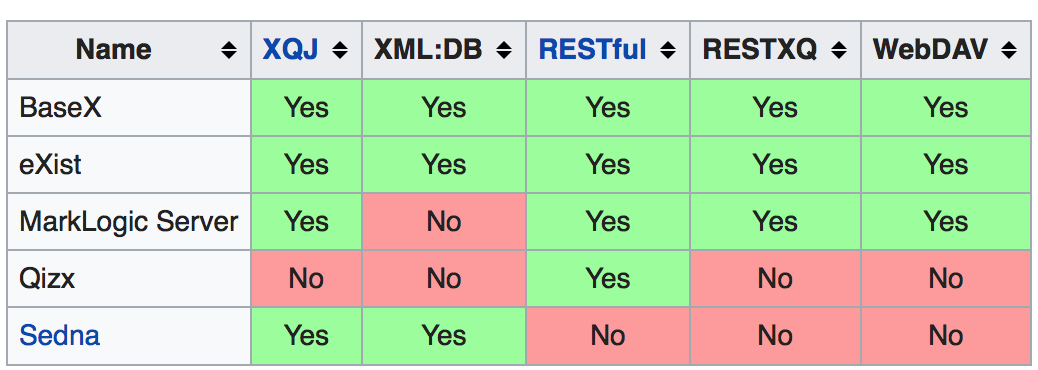
\includegraphics[width=\textwidth]{figures/XML_apis.png}
\end{column}
\end{columns}

\vskip1em

Unlike with relational data, however, XML systems must also expose them as documents which can be opened, edited, and saved by XML (file) editors. 

\end{frame}

\begin{frame}[fragile]{XQJ: XQuery API for Java}

XQJ was developed by the Java community and backed by major vendors (including Oracle and IBM); it became a standard in 2009. 

\bgroup
\lstset{
	language=Java,
	basicstyle=\ttfamily\scriptsize,
	commentstyle=\color{fern},
	stringstyle=\color{stringColor},
	keywordstyle=\sffamily\color{functionColor},
	emphstyle=[1]\color{datatypeColor},
	emph=[1]{conn,expr,result},
	emphstyle=[2]\color{blue},
	emph=[2]{getItemAsString,XQExpression,XQConnection,createExpression,close}
}

\begin{lstlisting}
// Create a new connection to an XML database
XQConnection conn = vendorDataSource.getConnection("myUser", "myPassword");

XQExpression expr = conn.createExpression(); // reusable XQuery Expression

XQResultSequence result = expr.executeQuery(
  "for $n in fn:collection('catalog')//item " +
  "return fn:data($n/name)"); // execute an XQuery expression

// Process the result sequence iteratively
while (result.next()) {
  // Print the current item in the sequence
  System.out.println("Product name: " + result.getItemAsString(null));
}

// Free all resources created by the connection
conn.close();
\end{lstlisting}
\egroup

\end{frame}

\begin{frame}[fragile]{Parameterized XQuery}

As with SQL, programs can pass parameters to an XQuery processor at runtime, via \textbf{external variables} in the query.

\bgroup
\lstset{
	language=Java,
	basicstyle=\ttfamily\scriptsize,
	commentstyle=\color{fern},
	stringstyle=\color{stringColor},
	keywordstyle=\sffamily\color{functionColor},
	emphstyle=[1]\color{datatypeColor},
	emph=[1]{conn,expr,result},
	emphstyle=[2]\color{blue},
	emph=[2]{getItemAsString,XQExpression,XQConnection,createExpression,close},
	moredelim = [is][\color{purple}\ttfamily]{-:}{:-}
}

\begin{lstlisting}
XQExpression expr = conn.createExpression();

// The XQuery expression to be executed
String es = -:"declare variable $x as xs:integer external;":- +
            " for $n in fn:collection('catalog')//item" +
            " where $n/price <= $x" +
            " return fn:data($n/name)";

// Bind a value (21) to an external variable with the QName x
expr.bindInt(new QName("x"), 21, null);

// Execute the XQuery expression
XQResultSequence result = expr.executeQuery(es);

while (result.next()) {
  // Process the result ...
}
\end{lstlisting}
\egroup
\end{frame}

\begin{frame}{XQJ Adoption}

Although not the only XQuery API out there, XQJ\footnote{\url{https://en.wikipedia.org/wiki/XQuery_API_for_Java}} is well supported.

\begin{itemize}[-]
\item \alert{File-based XQuery Processors}: Saxon XSLT and XQuery processor, \textcolor{blue}{Zorba}, MXQuery, Oracle XQuery Processor.

\item \alert{Native Systems}: MarkLogic, eXist, BaseX, Sedna, Oracle XDB, Tamino, TigerLogic, ...

\item \alert{Relational Systems}: Oracle DB (Not XDB), IBM DB2, Microsoft SQL Server, Sybase ASE, Informix, \textcolor{gray}{MySQL}, \textcolor{blue}{PostgreSQL}
\end{itemize}

Supporting= relational systems is not easy, because each implements XML in a different way. 
\end{frame}

\begin{frame}{ACID Transactions with XQJ}

From their manual (coloring added):

\vskip1em

\begin{quote}
By default a connection operates in auto-commit mode, which means that \alert{each XQuery is executed and committed in an individual transaction}. If auto-commit mode is disabled, a transaction must be ended explicitly by the application calling commit() or rollback().

An XQConnection object can be created on top of an existing JDBC connection. If an XQConnection is created on top of the JDBC connection, it inherits the transaction context from the JDBC connection.
\end{quote}

\end{frame}













